\begin{abstract}
	We present a platform for Melanoma Classification, leveraging a technical infrastructure based on Convolutional Neural Network (CNN) models. The models exclusively utilize image data, and no additional metadata is incorporated during the training process. Various training strategies were employed to enhance model performance.
	
	The resulting models are accessible through a  API, enabling users to interact with them via a straightforward web application. Users can submit batches of images to the API for classification, contributing to a user-friendly experience.
	
	This platform demonstrates the efficacy of CNNs in melanoma classification, highlighting the importance of diverse training approaches. The API provides a practical interface for users to seamlessly integrate melanoma classification into their workflows.
\end{abstract}


\section{Introduction}

Skin cancer, including melanoma, is a significant global public health concern.
Melanoma presents a considerable challenge due to its high mortality rate and
the critical importance of early detection for successful treatment. Cancer
begins when healthy cells undergo changes that cause them to grow and divide
uncontrollably, forming tumors. These tumors can be classified as either
cancerous (malignant) or non-cancerous (benign).\\

In recent times, there has been a growing focus on automating tasks in the
medical field through Computer-Aided Diagnosis (CAD)\footnote{CAD refers to the
use of computer algorithms and technologies to assist healthcare professionals
in the process of medical diagnosis.}. Some studies have demonstrated that
these systems can achieve results similar to those of professionals. However,
the integration of CAD into the medical system remains a significant challenge. \\

The development of a CAD system necessitates the creation of models capable of effectively classifying melanoma. The SIIM-ISIC Melanoma Classification challenge specifically tasks participants with building models for identifying melanoma using skin lesion images and associated metadata. This thesis outlines our approach, wherein we leverage data from this challenge to train our models and subsequently expose them through our platform. By doing so, we contribute to the ongoing efforts to bridge the gap between cutting-edge medical imaging technology and practical clinical applications.

\newpage

\section{Objectives}

The final objective of this thesis is to craft a CAD infrastructure,
focused on melanoma detection using deep learning vision models capable of detecting melanoma on dermoscopy images. To this end, the gradual achievements that
must be accomplished are:

\begin{itemize}

  \item Gaining a comprehensive understanding of the theory
    behind deep learning vision models and its practical applications.
    
   \item Select a base transfer model. Figuring out why, is this base model enough for our thesis?, the selection of this model is given by the technical limitations?, or any other justification.

  \item Study different approaches to train the models and select a good  evaluate metric given the dataset distribution of dermoscopy images.

  \item  Develop the CAD infrastructure. It should contain
    the  trained models, a simple web UI\footnote{User Interface. Is
    the point of human-computer interaction and communication in a device.}, an
    API\footnote{Application Programming Interface. Is a set of protocols,
      routines, tools, and definitions that allow different software applications
    to communicate with each othe} and finally a mechanism using Docker to create
    the images of these services making it ease to deploy in any based Linux System.

\end{itemize}


\section{Development Process}

The project methodology employed in this endeavor follows a continuous process.
The project incorporates the concept of utilizing idle time effectively. For
instance, during the training of models, there are periods of idle time, which
we exploited by concurrently working on other tasks related to developing the
entire infrastructure. This approach allows for maximizing productivity
throughout the project (see Figure \ref{fig:flux_development}).

\newpage

\begin{landscape}

  \begin{figure}[H]
  \centering
  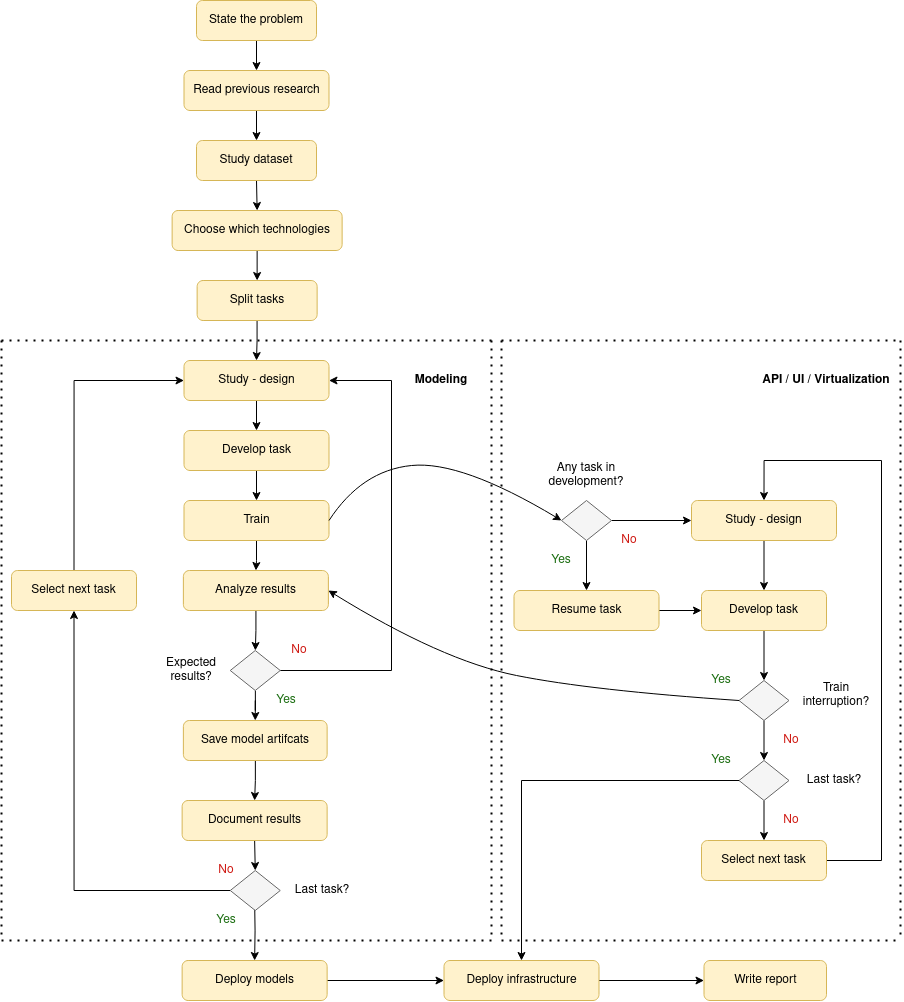
\includegraphics[width=0.82\textwidth]{imatges/planing_and_methodology/EmplyedMethodology.png}
  \caption{Activity diagram describing the methodology.}
  \label{fig:flux_development}
  \end{figure}

\end{landscape}


The process used to train, validate, test, and implement the models is
illustrated in Figure \ref{fig:cad-infrastructure-training-system}. This
sequence consists of several stages elaborated below. \\

The first stage involves cleaning and splitting the initial dataset into
smaller datasets. This step ensures that the data is organized and ready for
further processing. \\

The second stage focuses on training and validating the models using the
training and validation datasets. During this stage, the system reads images
and applies data augmentation techniques to train images and Test Time
Augmentation (TTA) to validation images. These techniques enhance the model's
performance by introducing variations in the data and improving its
generalization ability. \\

The third stage involves analyzing the training results obtained from different
training approaches. In this section*, we evaluate and analyze the model's
performance by comparing the predicted results against the test dataset. This
step helps us understand how well the models are learning and performing on
unseen data. \\

The last stage revolves around exposing the trained models through an API's
container image. This container image allows for easy deployment and
integration of the models into other systems or applications, providing a
convenient way to utilize the trained models for various tasks. \\


\begin{figure}[H]
  %\begin{adjustbox}{width=\textwidth, trim={0.2cm 0pt 1.5cm 0pt}, clip}
  \centering
  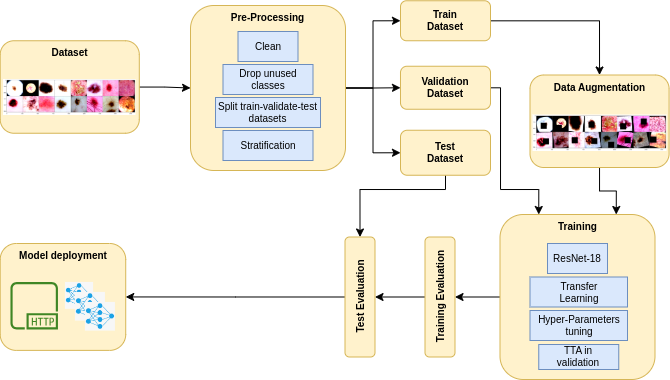
\includegraphics[width=0.9\textwidth]{imatges/methodological_contribution/Pipeline.drawio.png}
  %\end{adjustbox}
  \caption[CAD infrastructure pipeline]{\textit{CAD infrastructure pipeline. }}
  {\label{fig:cad-infrastructure-training-system}}
\end{figure}

\section{Results}

The training phase ended with the development of eight models using an
imbalanced dataset comprising eight classes. Various learning policies and
Artificial Intelligence (AI) techniques were tested during the experimentation
process.  \\

These models were divided into two categories: one without any
additional regularization and another with additional regularization techniques
such as data augmentation and the inclusion of dropout layers.

\begin{table}[H]
\centering
\begin{tabular}{lc|lc}
    \toprule
  \textbf{Model} & \textbf{Test AUC} & \cellcolor{gray!50}\textbf{Model} & \cellcolor{gray!50}\textbf{Test AUC}  \\
\midrule
 M0 & 0.892 & \cellcolor{gray!50}M4 & \cellcolor{gray!50}0.858 \\
 M1 $\star$ & 0.892 & \cellcolor{gray!50}M5 $\star$ & \cellcolor{gray!50}0.843 \\
 M2 $\ast$ &  0.885 &  \cellcolor{gray!50}M6 $\ast$ & \cellcolor{gray!50}0.848 \\
 M3 $\bullet$ & 0.886 & \cellcolor{gray!50}M7 $\bullet$ & \cellcolor{gray!50}0.849 \\
 \midrule
Mean &  88.875\% & \cellcolor{gray!50}Mean & \cellcolor{gray!50}84.950\%  \\
SD &  0.377\%  &   \cellcolor{gray!50}SD &  \cellcolor{gray!50}0.625\%  \\

\bottomrule
\end{tabular}
\caption[Models metrics in test dataset]
  {\textit{Models metrics in test dataset.}}
{\label{table:test-set-resume-metrics}}
\end{table}

The initial group of models performed well on the test set with an average AUC
of 88.875\% and a small standard deviation of ±0.377\%. However, they showed
signs of overfitting on the validation set. In contrast, the second group of
models, trained with additional regularization techniques, achieved lower
results but did not suffer from overfitting. They had an average AUC of 84.950%
with a standard deviation of ±0.625\%, which was influenced by more training
epochs. \\

During model training, we also developed the necessary CAD infrastructure. For
the API, we used a flexible approach with soft configurations that could be
specified through file-based parameters, offering adaptability and simplified
management. Additionally, we created an intuitive UI for seamless interaction
between healthcare professionals and the models. \\

We also provided a Docker-based script for easy deployment of the
infrastructure on any Linux operating system, ensuring efficient startup and
operation.
